\section{分次环的\texorpdfstring{$\proj$}{Proj}}\label{s:3.2}

\subsection{\texorpdfstring{$\proj S$}{Proj S}的构造}\label{s:3.2.1}

到目前为止,非仿射概形最重要的例子是在一个仿射概形$\spec A$上的\textit{射影}概形,其中$A$是任意一个交换环。(为简单起见,我们常常说一个概形在$A$上射影,而不说在$\spec A$上射影。)这样的一个概形来自于一个分次$A$-代数,而构造过程非常类似于从它的齐次坐标环构造一个射影簇。我们可以从一个分次$\oo_B$-代数层开始,定义在任意的基概形$\spec B$上射影的概形,这个拓展有重要的应用。但对这个理论中的大部分情况而言,我们都可以将情况约化到$B$是一个仿射概形,故而在这里,我们对一般性的追求也仅止于此。

为了描述这个构造,我们从一个正分次$A$-代数开始,其中$A$作为这个代数的$0$次部分,即一个$A$代数$S$具有分次
\[
	S=\bigoplus_{\nu=0}^\infty S_\nu\quad \text{作为$A$-模}
\]
使得
\[
	S_\nu S_\mu \subset S_{\nu+\mu}\quad \text{以及} \quad S_0=A.
\]
$S$中的一个元素如果处于$S_\nu$中,则它被称为$\nu$\textit{次齐次}的。我们将从$S$定义一个$A$-概形$X=\proj S$. 在$A$上射影的概形就被定义为具有形式$\proj S$的概形,其中$S$是一个有限生成$A$-代数。代数$S$被称为$X$的\textit{齐次坐标环},尽管(类似于射影簇的齐次坐标环)实际上他并不由$X$所决定。

当$S$是$A$上的多项式环
\[
	S=A[\text{$x_0$, $\dots$, $x_r$}],
\]
具有如下分次:$A$中的元素是零次的,而每一个变量的分次都是$1$,则给出的概形$\proj S$被称为\textit{$A$上的射影$r$-空间},记作$\mathbb{P}_A^r$.(后面的习题将说明这个概形与第 \ref{chap:1} 章中定义的概形$\mathbb{P}_A^r$是相同的。)在$A=K$是一个域的例子中,概形$\mathbb P_K^r$与$K$上的名为射影空间的簇之间的关系就类似于概形$\mathbb A_K^r$与名为仿射$r$-空间的簇之间的关系。

为方便起见,我们将假设代数$S$在$A$上被它的$1$-次元素所生成,类似于多项式环那样,一般的情况我们留做习题。(换个方向,如果$S$并没有假设在$A$上有限生成,下面我们说的绝大部分内容依然成立,但这种推广用得相对较少)。

$\proj S$可以如下定义:对$S$中的正次齐次元生成的理想,我们记
\[
	S_+=\bigoplus_{\mu=1}^\infty S_\mu.
\]
我们称一个理想是\textit{齐次}的如果它由齐次元所生成。底空间$|\proj S|$是环$S$中所有不包含$S_+$的齐次素理想的集合(它们有时候被叫做\textit{相关}素理想,而$S_+$因此被叫做\textit{无关理想})。$|\proj S|$上的拓扑通过闭集定义,闭集取做形如
\[
	V(I):=\{\pp\,|\,\text{$\pp$是$S$的包含$I$的相关素理想}\}
\]
的集合,其中$I$是$S$的齐次理想。

我们将在开集基的每一个元素上明确$|\proj S|$的概形结构。为此,令$f$是$S$的任意$1$-次齐次元素,以及$U$是开集
\[
	|\proj S|-V(f),
\]
所有不包含$f$的齐次素理想(于是也不包含$S_+$)。$U$中的点可以等同于$S[f^{-1}]$中的齐次素理想。另一方面,这些齐次素理想关联于环$S[f^{-1}]$中所有的$0$次素理想,我们将其记作$S[f^{-1}]_0$,见Exercise \ref{exe:3.6}(a). 于是,我们可以将$U$与$\spec S[f^{-1}]_0$的拓扑空间相等同,然后给他一个相应的仿射概形结构。我们将用$(\proj S)_f$来记这些$\proj S$的仿射开子概形。如果$1$-次元$x_0$, $x_1$, $\dots$们生成了一个理想,它的根是无关理想$S_+$,于是开集
\[
	(\proj S)_{x_i}:=\proj S-V(x_i)
\]
就构成了$\proj S$的一个仿射开覆盖。

如果$g$是$S$的另一个$1$-次元,接着重叠部分$(\proj S)_f\cap (\proj S)_g$是$(\proj S)_f$的由
\[
	S[f^{-1}]_0[(g/f)^{-1}]=S[f^{-1},g^{-1}]_0
\]
的谱给出的仿射开集。因为上式关于$f$和$g$对称,所以我们有一个自然的等同
\[
	((\proj S)_f)_{(g/f)}=((\proj S)_g)_{(f/g)}.
\]
正如第 \ref{s:1.2.4} 节中讨论的黏合构造,它们将$\proj S$变为了一个概形。

在本节的剩余部分以及下节中,我们将展示一些射影概形的基本事实以及它们的闭子概形。因为这些事实以及它们的证明与簇的情况中的很类似,我们将它们留作习题。

\begin{exe}\label{exe:3.6}
\begin{compactenum}[(a)]
\item 对$S$任意的齐次理想$I$,以及$1$-次齐次元$f$,交集
\[
	(I\cdot S[f^{-1}])\cap S[f^{-1}]_0
\]
由一族$I$的齐次生成元乘以合适的$f$的(负的)次幂生成($f$是任意次的推广见 Exercise \ref{exe:3.10})。于是,$S[f^{-1}]$的齐次素理想一一对应于$S[f^{-1}]$的$0$-次元构成的环的素理想。对应由$S[f^{-1}]$的素理想$\pp$变为$\mathfrak q=\pp\cap S[f^{-1}]_0$给出,其逆为将$S[f^{-1}]_0$的素理想$\mathfrak{q}$变为$\mathfrak qS[f^{-1}]$.

\item 令$S=A[x_0$, $\dots$, $x_r]$为多项式环,而$U$是$\mathbb P_A^r=\proj S$的仿射开集$(\mathbb P_A^r)_{x_i}$. 由定义,
\[
	U=\spec S[x_i^{-1}]_0,
\]
证明
\[
	S[x_i^{-1}]_0=A[x'_0,\dots,x'_r]
\]
为生成元$x'_j=x_j/x_i$的多项式环。(注意$x'_i=1$,所以这是一个$r$变量的多项式环。)于是
\[
	(\mathbb P^r_A)_{x_i}=\mathbb A_A^r
\]
所以射影$r$-空间被$r+1$个仿射$r$-空间所覆盖,就像第 \ref{chap:1} 章中所描述的那样。

\item 考虑一个映射$\alpha:S\to S[x_i^{-1}]_0$,他将$x_i$变为$1$以及对$j\neq i$将$x_j$变为$x'_j$. 从(a)证明如果$I$是$S$的一个齐次理想,于是
\[
	I':=I\cdot S[x_i^{-1}]\cap S[x_i^{-1}]_0=\alpha(I)'\cdot S[x_i^{-1}]_0.
\]
从$I$构造$I'$的过程被称为\textit{非齐次化}。像经典的那样,描述与其相反的过程,齐次化。
\end{compactenum}
\end{exe}

\nottran

\begin{center}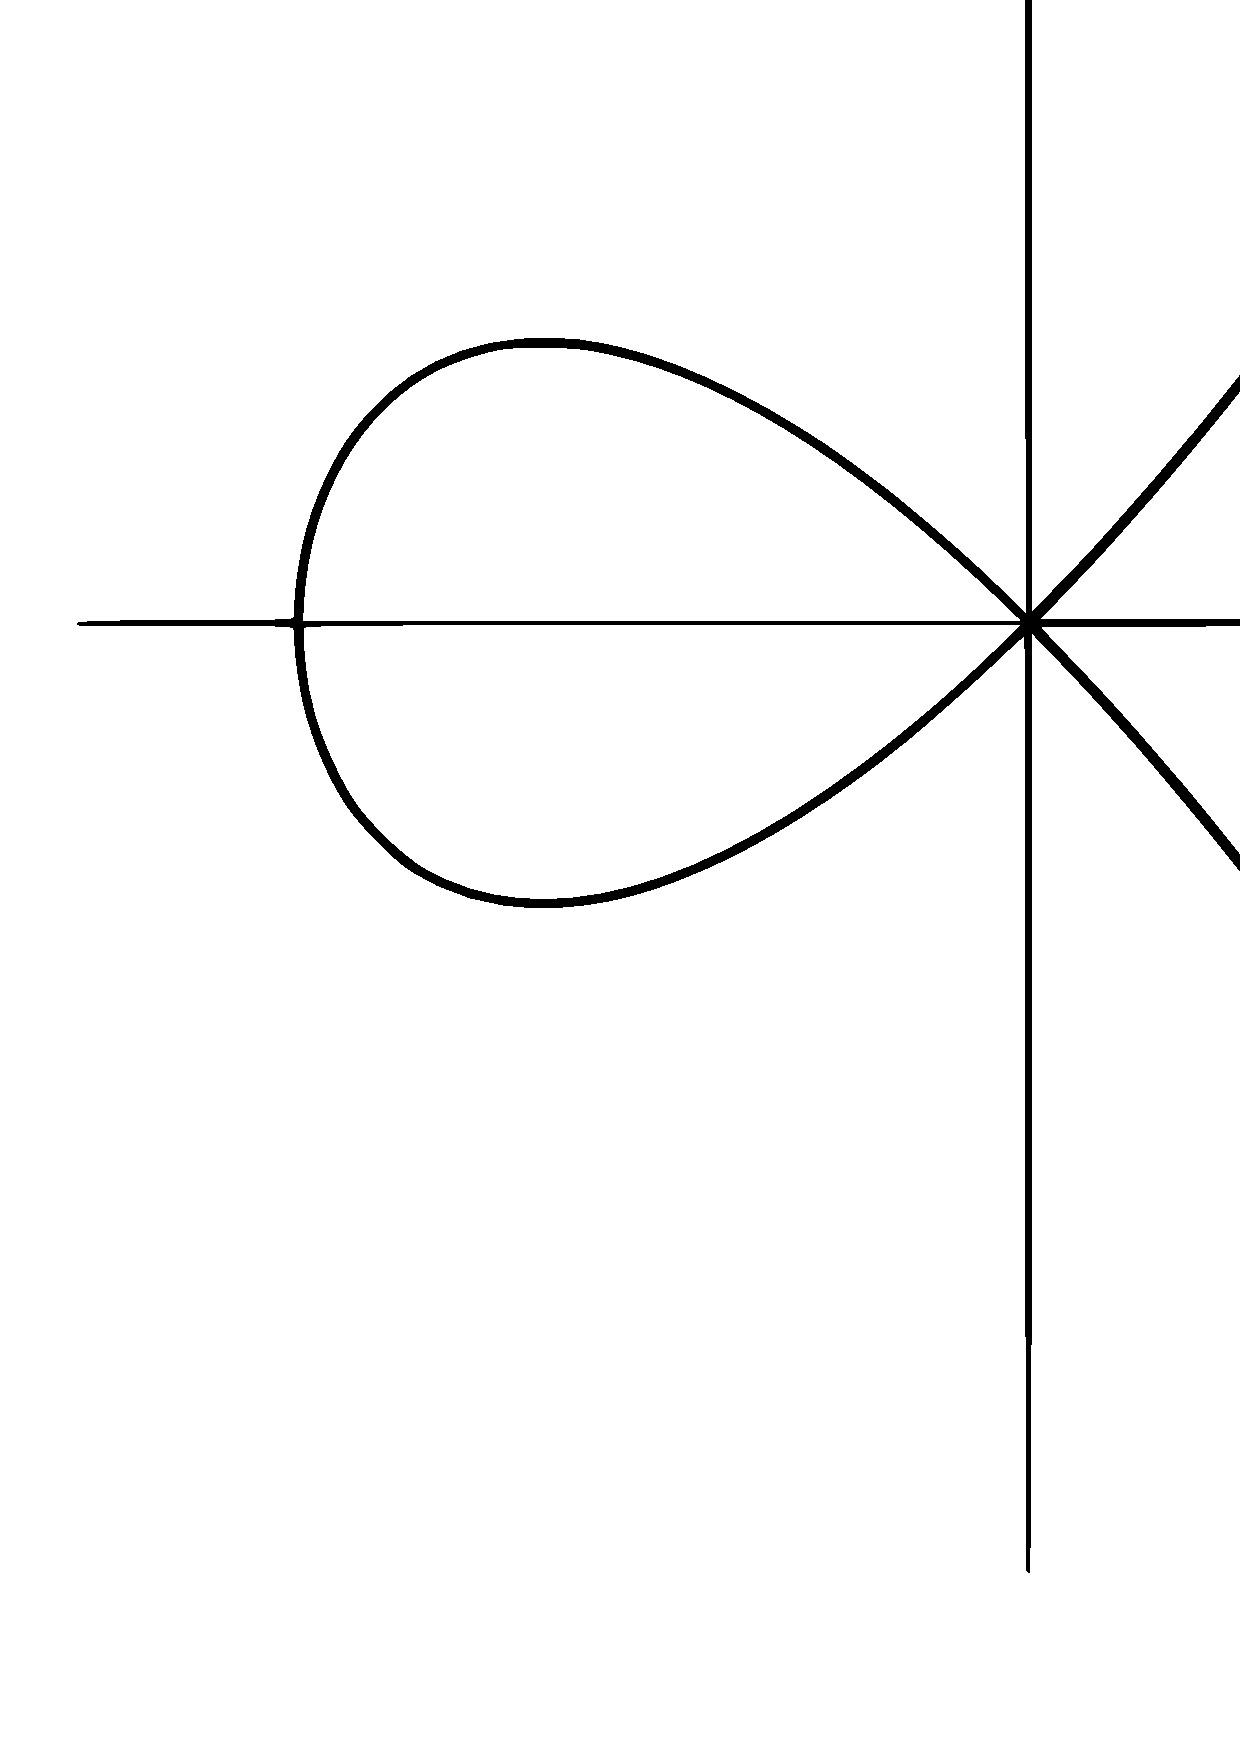
\includegraphics[scale=\scale,bb=0 0 668 462]{\PICDIR/2.png}\end{center}

\begin{exe}\label{exe:3.9}
在上图中添入点$(4x_1-5x_0)$, $(2x_1-5x_0)$以及$(5)$的闭包(可以与第 \ref{s:2.4.3} 节中的$\mathbb A_{\mathbb Z}^2$的图相比较)。\textit{注意}:曲线$(4x_1-5x_0)$应该画得与“位于$\infty$的点”$(x_0)$相切,而曲线$(2x-5x_0)$不能。通俗地,我们可以说这是因为函数$5/4$在$(2)$处有一个双极点,而$5/2$只有一个单极点。(同样可见 Exercise \ref{exe:2.38} 中的讨论。)
\end{exe}

\begin{exe}\label{exe:3.10}
按上面的记号,令$h$为$S$的一个正次齐次元。集合
\[
	(\proj S)_h:=\proj S-V(h)
\]
同前为$S$中不包含$h$的齐次素理想构成的集合。证明这个集合依然一一对应于$S[h^{-1}]_0$的素理想,所以实际上存在一个$\spec S[h^{-1}]_0$与$\proj S$的(仿射)开子概形的同构。同样证明,这样的仿射开集族
\[
	\{(\proj S)_h\}_{h\in H}
\]
是一个$\proj S$的开覆盖,当且仅当$H$的元素生成了一个根为$S+$的理想。
\end{exe}

\begin{exe}\label{exe:3.11}
推广$\proj S$的定义到$S$不被$1$-次元所生成的情况,以及证明$\proj S$是一个射影概形。
\end{exe}

\begin{exe}\label{exe:3.12}
令$S$是一个分次环,没必要是有$1$-次元生成的。对任意的正次$d$,定义$S$的$d$-次\textit{Veronese 子环}为分次环
\[
	S^{(d)}=\bigoplus_{\nu=1}^\infty S_{d\nu}
\]
证明$\proj S$同构于$\proj S^{(d)}$. 然而,证明如果$S=A[x,y]$,则$S^{(d)}$作为分次代数(甚至仅作为环)并不同构于$S$. 于是,就像在簇中那样,分次代数与射影概形的对应并不是一一的。
\end{exe}

\subsection{\texorpdfstring{$\proj R$}{Proj R}的闭子概形}\label{s:3.2.2}

一个齐次理想$I\subset A[x_0$, $\dots$, $x_r]$确定了一个凝聚理想层$\tilde I\subset \mathscr O_{\mathbb P_A^r}$,因而一个$\mathbb P_A^r$的闭子概形。下面的习题建立了这些事实。

\begin{exe}
对每个开集
\[
	U_i=(\mathbb P_A^r)_{x_i}=\spec A[x_0,\dots,x_r,x_i^{-1}]_0\cong \mathbb A_A^r,
\]
令$\tilde I(U_i)$为理想$I\cdot A[x_0,\dots,x_r,x_i^{-1}]\cap A[x_0,\dots,x_r,x_i^{-1}]_0$. 证明这个定义可以以唯一的方式拓展到其他开集$U$上使得$\tilde{I}$成为一个凝聚理想层。
\end{exe}

\begin{defi}
一个概形间态射$\varphi:X\to Y$被称为\textit{射影}的,如果他是一个闭嵌入$X\to \mathbb P_Y^n$和结构态射$\mathbb P_Y^n\to Y$的复合。
\end{defi}

注意到,如果$Y=\spec A$是仿射的,这相当于说$X$具有形式$\proj S$,其中$S$是一个有限生成$A$-代数。射影态射的基本事实前面已经说过了:

\begin{thm}
射影态射是逆紧的。
\end{thm}

证明可见Hartshorne [1977, Theorem II.4.9].

\subsection{整体\texorpdfstring{$\proj$}{Proj}} \label{s:3.2.3}
\subsection{切空间和切锥} \label{s:3.2.4}
\subsection{到射影空间的态射} \label{s:3.2.5}
\subsection{分次模和层} \label{s:3.2.6}
\subsection{Grassmann流形} \label{s:3.2.7}
\subsection{全景超曲面} \label{s:3.2.8}
